\documentclass[12pt,a4paper]{article}
\usepackage[italian]{babel}
\usepackage[T1]{fontenc}
\usepackage[latin1]{inputenc}
\usepackage{graphicx}
\usepackage{amsmath}
\usepackage{subfig}
\usepackage[a4paper,top=1.5cm,bottom=1.4cm,left=1.4cm,right=1.4cm]{geometry}
\date{}
\begin{document}
\title{Aeroelasticit�\\ Esercitazione 4 \\ Prof.re Franco Mastroddi}
\author{Matteo Hakimi\\ 1455230}
\maketitle
\begin{figure}[htbp]
\centering

\includegraphics[width=100mm]{Immagini/1}
\end{figure}
\newpage
\tableofcontents
\newpage

\section{Introduzione}
 Si vuole studiare la stabilit� di una superficie portante sottile investita da una corrente, attraverso l'uso del solutore SOL 145 del codice NASTRAN. In particolare verranno calcolate le velocit\'a di {\itshape divergenza} e {\itshape flutter} e il luogo delle radici del sistema preso in considerazione. 
\section{Formulazione del problema}
La superficie portante viene modellata come se fosse una lastra piana rigida collegata elasticamente alla fusoliera, attraverso degli elementi cedevoli.\\
In particolare le rigidezze flessionale e torsionale della struttura vengono sostituite con delle molle concentrate, applicate, ad un estremo, al punto di ascissa $x_{e}$,  corrispondente al centro elastico di questa, e, all'altro estremo, alla fusoliera (si veda figura 1).\\
\begin{figure}[htbp!]
	\centering	
	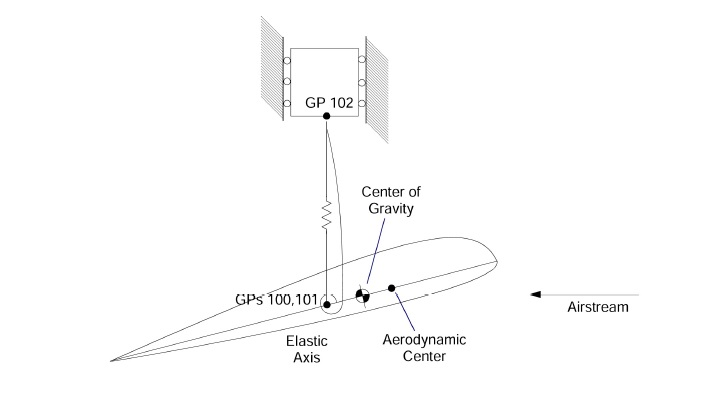
\includegraphics[width=100mm]{Immagini/profilo}
	\caption{Sezione tipica vincolata elasticamente alal fusoliera}
\end{figure}\\
Dove la fusoliera � libera solo di traslare verticalmente.\\
I gradi di libert� scelti per descrivere il problema sono: lo spostamento verticale (T3) di un punto della superficie portante ({\itshape plunge}), la rotazione attorno al centro di massa del profilo (R2) e il {\itshape plunge} della fusoliera (T3).\\
\subsection{Implementazione del modello}

Il file .dat, che deve essere implementato al fine dell'analisi in ambiente NASTRAN, consta di tre sezioni principali: l'{\itshape Executive Control Section}, il {\itshape Case Control Section} e il {\itshape Bulk Data Section}; nella prima scheda, deve essere  specificato il tipo di solutore utilizzato nell' analisi.\\ Quest'ultimo dipende dal tipo di problema preso in considerazione; nel caso del {\itshape flutter} si ha: SOL 145.\\
Nel {\itshape Case Control Section} vengono indicati i metodi numerici utilizzati per la risoluzione del problema preso in considerazione. Nella fattispecie, si \'e scelto il metodo p-k per il problema aeroelastico; mentre per il calcolo degli autovalori/autovettori, del problema di dinamica strutturale, si \'e fatto uso del metodo di {\itshape Lanczos}.\\
Infine nella terza parte viene riportato il modello aeroelastico in questione, comprensivo delle sue caratteristiche aerodinamiche e strutturali.\\
Da quanto detto sopra, al fine del calcolo della stabilit\'a aeroelastica, dobbiamo innanzitutto introdurre un modello strutturale, che ci permetta di calcolare i modi propri, e relative frequenze proprie, della struttura. Ricordiamo infatti, come il sistema di equazioni del moto, e relative condizioni al contorno, sia ottenuto a partire dalla proiezione dell'equazione di Cauchy sulle funzioni di forma, scelte coincidenti con i modi propri della struttura.\\
Un modello strutturale semplice proposto, viene mostrato in figura 2: \\
\begin{figure}[htbp!]
	\centering	
	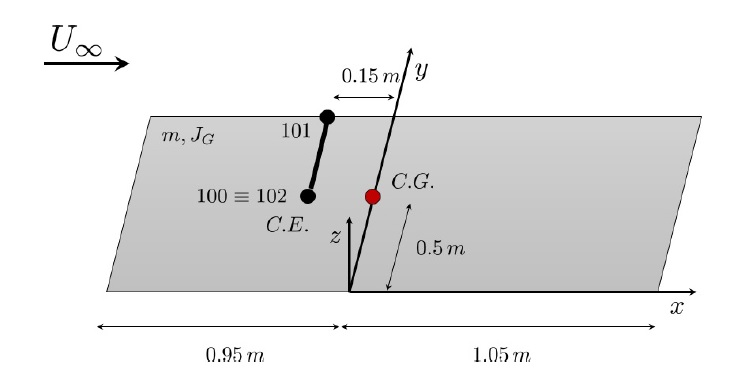
\includegraphics[width=100mm]{Immagini/profilo2}
	\caption{Modello strutturale della sezione tipica}
\end{figure}\\
dove:\\\\
$\bullet$\quad C.E= il centro elastico\\
$\bullet$\quad C.G= il centro di massa coincidente con l'origine del sistema di riferimento scelto\\\\
In particolare i gradi di libert\'a della struttura, superficie portante e fusoliera, \'e descritto attraverso l'utilizzo di 3 nodi (GRID) e di un elemento rigido di collegamento RBAR:\\\\
$\bullet$\quad GRID 100 posto sulla {\itshape centerline} del profilo in corrispondenza del C.E.\\
$\bullet$\quad GRID 102 coincidente con GRID 100 rappresentante la fusoliera.\\
$\bullet$\quad GRID 101 connesso al GRID 100 attraverso l'elemento rigido RBAR 101.\\\\
Per poter modellizzare il comportamento elastico della struttura, vengono posti degli elementi CELAS2, che rappresentano degli elementi ad elasticit\'a concentrata.\\
In particolare, viene posto un elemento CELAS2, che definisce il comportamento flessionale, tra la fusoliera (GRID 102) e il profilo (GRID 100), e un'altro posto tra il profilo (GRID 100) e il terreno, a simulare la molla di torsionale.\\
Infine per tener conto delle propriet\'a inerziali, della superficie portante e della fusoliera, vengono posti degli elementi CONM2 e CMASS2. In particolare l'elemento CONM2 viene posto in corrispondenza del centro di massa del profilo, in modo da tener conto della massa $m_{a}$ e del tensore di inerzia ($I_{22}$) dello stesso; mentre l'elemento CMASS2 viene posto in corrispondenza del GRID 102 e rappresenza la massa $M_{f}>>m_{a}$ della fusoliera.\\
Come precedentemente detto, nel Bulk Data Section, oltre a definire la struttura e le sue caratteristiche, viene definito il modello aerodinamico. In particolare nella card AERO sono specificati la velocit\'a di riferimento, la densit\'a del flusso e la corda.\\
Mentre nelle cards CAERO4 e PAERO4, vengono definite le caratteristiche aerodinamiche della struttura. In particolare, nel caso preso in considerazione, il modello aerodinamico si basa sulla {\itshape Strip theory}, ovvero la superficie portante viene schematizzato come un singolo pannello, di profondit\'a 1 in direzione y (si veda figura 2), in cui la soluzione viene rappresentata dalla teoria di {\itshape Theodorsen} esatta, avendo trascurato gli effetti di comprimibilit\'a.\\
A questo punto bisogna associare le caratteristiche aerodinamiche alla superficie portante, generando un pannello a partire dalla modellizzazione della struttura, nella parte dedicata della {\itshape Bulk Data Section}; Questa operazione viene effettuata mediante l'interpolazione della struttura attraverso delle {\itshape Spline function}.\\
Nella sezione MKAERO1 viene generata la matrice delle forze aerodinamiche generalizzate GAF, costruita, per interpolazione, a partire dai valori campionati dalla valutazione della stessa, per una certa frequenza ridotta e per un certo numero di Mach, avendo definito un set di valori a priori per quest'ultimi.\\
Infine nella scheda FLFACT, viene specificato il range di densit\'a del fluido preso in considerazione, la velocit\'a di {\itshape free stream} e il numero di Mach, che bisogna considerare nell'analisi di stabilit\'a.\\
Nella fattispecie l'analisi di stabilit\'a verr\'a condotta a quota fissa ($\rho= costante$) e a numero di Mach costante e pari a zero (flusso incomprimibile). Verr\'a invece fatta variarare la velocit\'a della corrente indisturbata.\\
Scegliendo una condizione di volo al livello del mare $\rho=1.22$ $\frac{kg}{m^3}$, assumendo come parametri non dimensionali, descrittivi della nostra superficie portante, coincidenti con quelli dell' {\itshape Esercitazione 2}:\\
$$a=5,\quad \Omega=0.5,\quad \xi_{E}=0.30,\quad \xi_{G}=0.45,\quad r_{\alpha}^2=0.25$$  
caratterizziamo il problema per un profilo che presenti le seguenti caratteristiche:\\
$$b=2m,\quad \omega_{\alpha}=100 rad/s$$ 
Da cui si ricava:\\
$\bullet$\quad $m_{a}=a\rho\pi b^2=19.16$ $kg$\\
$\bullet$\quad $J_{\alpha}=4.7909$ $kg m^2$\\
$\bullet$\quad $J_{G}=J_{\alpha}-m(x_{G}-x_{E})^2=4.3501$ $kg m^2$\\
$\bullet$\quad $k_{h}=m\omega_{h}^2=47909$ $N/m$\\ $\bullet$\quad$k_{\alpha}=m\omega_{\alpha}^2=47909$ $N/m$\\

dove:\\\\
$\bullet$\quad $m_{a}$ � la massa del profilo\\
$\bullet$\quad $J_{\alpha}$ il momento di inerzia calcolato rispetto al centro elastico C.E.\\
$\bullet$\quad $J_{G}$ il momento di inerzia calcolato rispetto al centro di massa C.G. \\
$\bullet$\quad $k_{h}$ la rigidizza flessionale del sistema pensato disaccoppiato\\
$\bullet$\quad $k_{\alpha}$ la rigidizza torsionale del sistema pensato disaccoppiato\\
Mentre per quanto riguarda la massa della fusoliera, abbiamo che $M_{f}=99999999$ $kg$\\
Prima di procedere con lo studio della stabilit� del sistema, � opportuno precisare che nell'analisi modale della struttura � stato richiesto il calcolo dei primi 6 modi di vibrare, anche se, al fine dell'analisi aeroelastica sarebbero stati sufficienti un numero pari a 3. Il fatto che si richieda il calcolo di un numero maggiori di modi strutturali rispetto a quelli sufficienti, � legato all'accuratezza della soluzione che si vuole ottenere.\\
\newpage
\section{Stabilit� aeroelastica}
In questa sezione si vuole studiare, attraverso l'uso del luogo delle radici, la stabilit� del sistema.\\
Una volta implementato il modello nel file .dat, viene effettuato il run su codice NASTRAN che fornisce i risultati nel file f06, in cui si � scelto, al fine dell'analisi di stabilit�, un intervallo di velocit� dimensionale pari a $40\div 150$ $m/s$ .\\
In particolare, dalla tabella denominata {\itshape Flutter summary}, contenuta nell' f06, � possibile ottenere il luogo delle radici dimensionale costruito al variare della velocit�.\\
Viene qui riportato il luogo delle radici, graficato grazie all'ausilio di uno script realizzato in ambiente Matlab.\\
\begin{figure}[htbp!]
	\centering	
	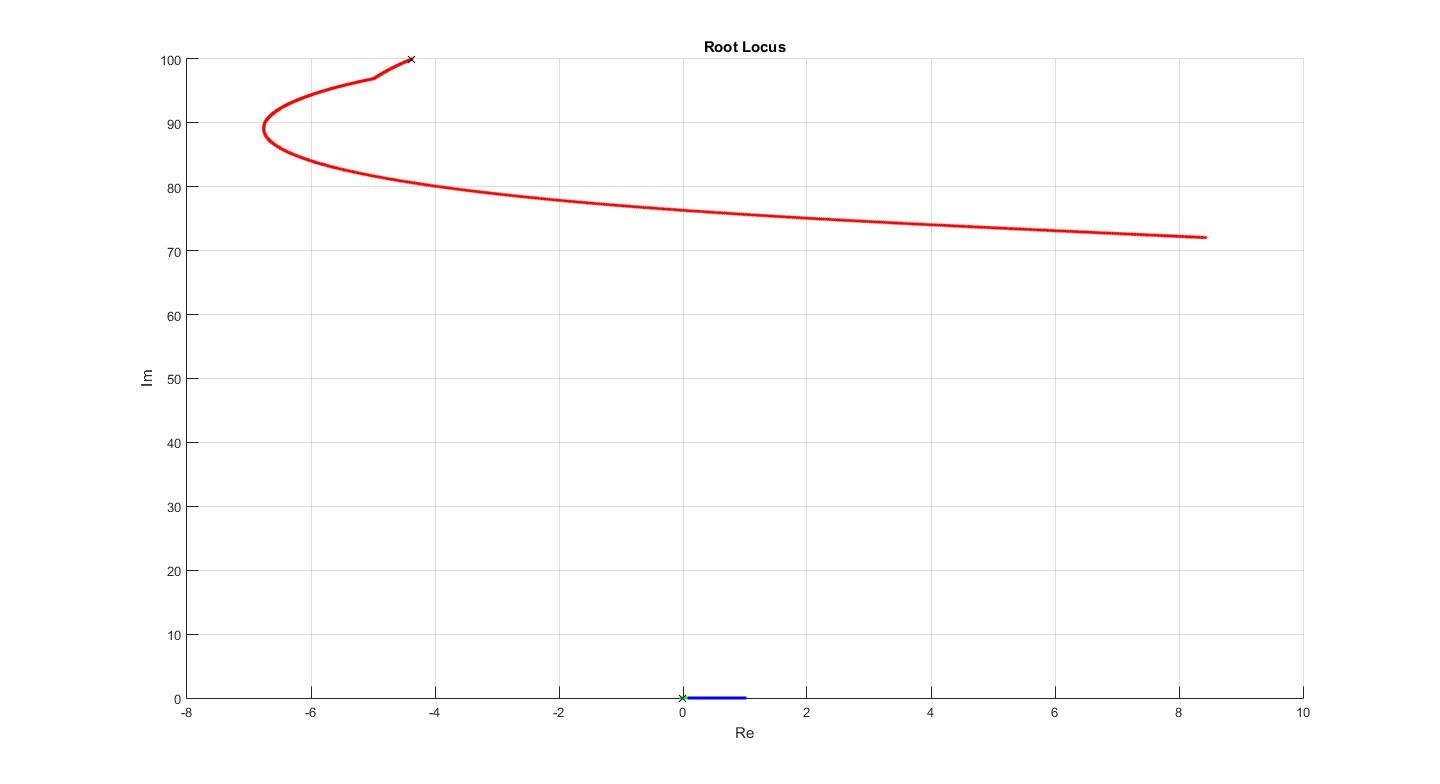
\includegraphics[width=150mm]{Immagini/rlocus}
	\caption{Luogo delle radici della sezione tipica}
\end{figure}\\
Sul luogo delle radici, si osserva la presenza di 3 poli, corrispondenti ai 3 gdl utilizzati per descrivere il moto del sistema.\\ In particolare in corrispondenza dell'origine si nota un polo fisso, al variare della velocit� $U$, contrassegnato di verde (si veda figura), corrispondente al moto rigido della stuttura.\\ Per quanto riguarda gli altri poli, si osserva come questi entrambi attraversano l'asse immaginario. In particolare si osserva come il polo a frequenza maggiore attraversi l'asse immaginario a una determinata frequenza; mentre quello delineato in blu lo attraversi nell'origini. Le due situazioni, appena descritte, corrispondono al fenomeno di divergenza aeroelastica di {\itshape flutter} e {\itshape divergenza} rispettivamente.\\
\newpage
Al fine di individuare i valori di velocit� dimensionale corrispondenti alle due situazione sopra citate, si riporta in figura sottostante l'andamento dello smorzamento al variare della velocit� dimensionale.\\
I valori critici, vengono individuati attraverso il cambio di segno dello stesso al variare di $U$.\\
\begin{figure}[htbp!]
	\centering	
	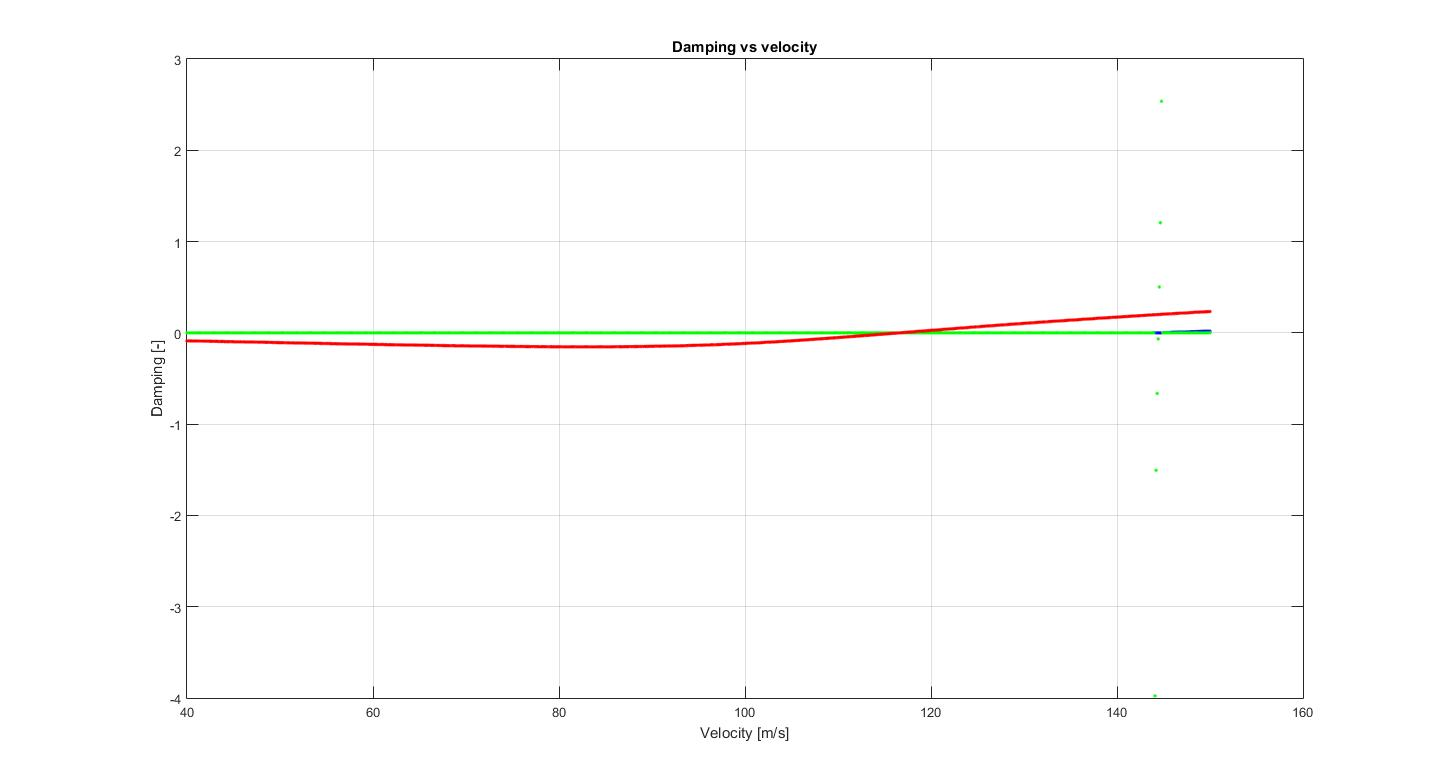
\includegraphics[width=150mm]{Immagini/dvsv}
	\caption{Andamento dello smorzamento al variare della velocit� }
\end{figure}\\  
Dal grafico di figura si ricava:\\
\begin{center}
	\begin{tabular}{c c}
		\hline
		$U_{F}=$&116.62 $m/s$\\
		\hline
		$U_{D}=$&144.78 $m/s$ \\					
		\hline
	\end{tabular}
\end{center}
Ricordando che:
$$\hat{U}=\frac{Ub}{\omega_{\alpha}}$$
si ottiene:\\
\begin{center}
	\begin{tabular}{c c}
		\hline
		$\hat{U}_{F}=$&1.166 \\
		\hline
		$\hat{U}_{D}=$&1.447 \\					
		\hline
	\end{tabular}
\end{center}
Per il caso di divergenza dinamica, viene riportato anche il valore della frequenza ridotta corrispondente:\\
$$k=0.6541$$	
\newpage
\section{Confronti dei risultati con esercitazione 3}
In questa sezione viene effettuato il confronto, in termini di velocit� adimensionali e frequenze ridotte critiche, ottenute nell' {\itshape Esercitazione 3}.
Vengono riportati in tabella i relativi casi con i valori critici ottenuti, sia nel caso di divergenza aeroelastica che nel flutter.\\
Indicato con:\\\\          
$\bullet$\quad {\bf ANSS}= Aerodinamica non stazionaria, struttura smorzata.\\
$\bullet$\quad {\bf AQSNS}$_{Th}$= Aerodinamica quasi-stazionaria, struttura non smorzata, modello $\tilde{C}_{k}\rightarrow1$.\\
$\bullet$\quad {\bf AQSS}$_{Th}$= Aerodinamica quasi-stazionaria, struttura smorzata, modello $\tilde{C}_{k}\rightarrow1$. \\
i casi trattati nella terza esercitazione si ha:\\\\

\begin{center}
	\begin{tabular}{lcccc}
		\hline
		\hline
		{\bf Caso} & $k_{F}$& $U_{F}$& $k_{D}$& $U_{D}$\\
		\hline
		{\bf ANSS}&0.6557&1.1701&0&1.4426\\
		\hline
		{\bf AQSNS}$_{Th}$&5.9731&0.1790&0&1.4430\\
		\hline
		{\bf AQSS}$_{Th}$&1.6408&0.6087&0&1.4434\\
		\hline
		\hline
	\end{tabular}
\end{center}
Mentre nella sezione precedente abbiamo ottenuto:\\
\begin{center}
	\begin{tabular}{c c}
		\hline
		$k_{F}=$&0.6541\\
		\hline
		$\hat{U}_{F}=$&1.166 \\
		\hline
		$k_{D}=$&0\\
		\hline
		$\hat{U}_{D}=$&1.447  \\					
		\hline
	\end{tabular}
\end{center}
Si noti come la soluzione ottenuta tramite codice NASTRAN sia molto simile a quella ottenuta analiticamente nel caso di aerodinamica non stazionaria con struttura non smorzata.\\
 Questo a ragione di aver implementato la funzione esatta di {\itshape Theodorsen} sul singolo pannello, e aver considerato la struttura non smorzante.\\





\end{document}